

\begin{figure}[p]
    \centering
    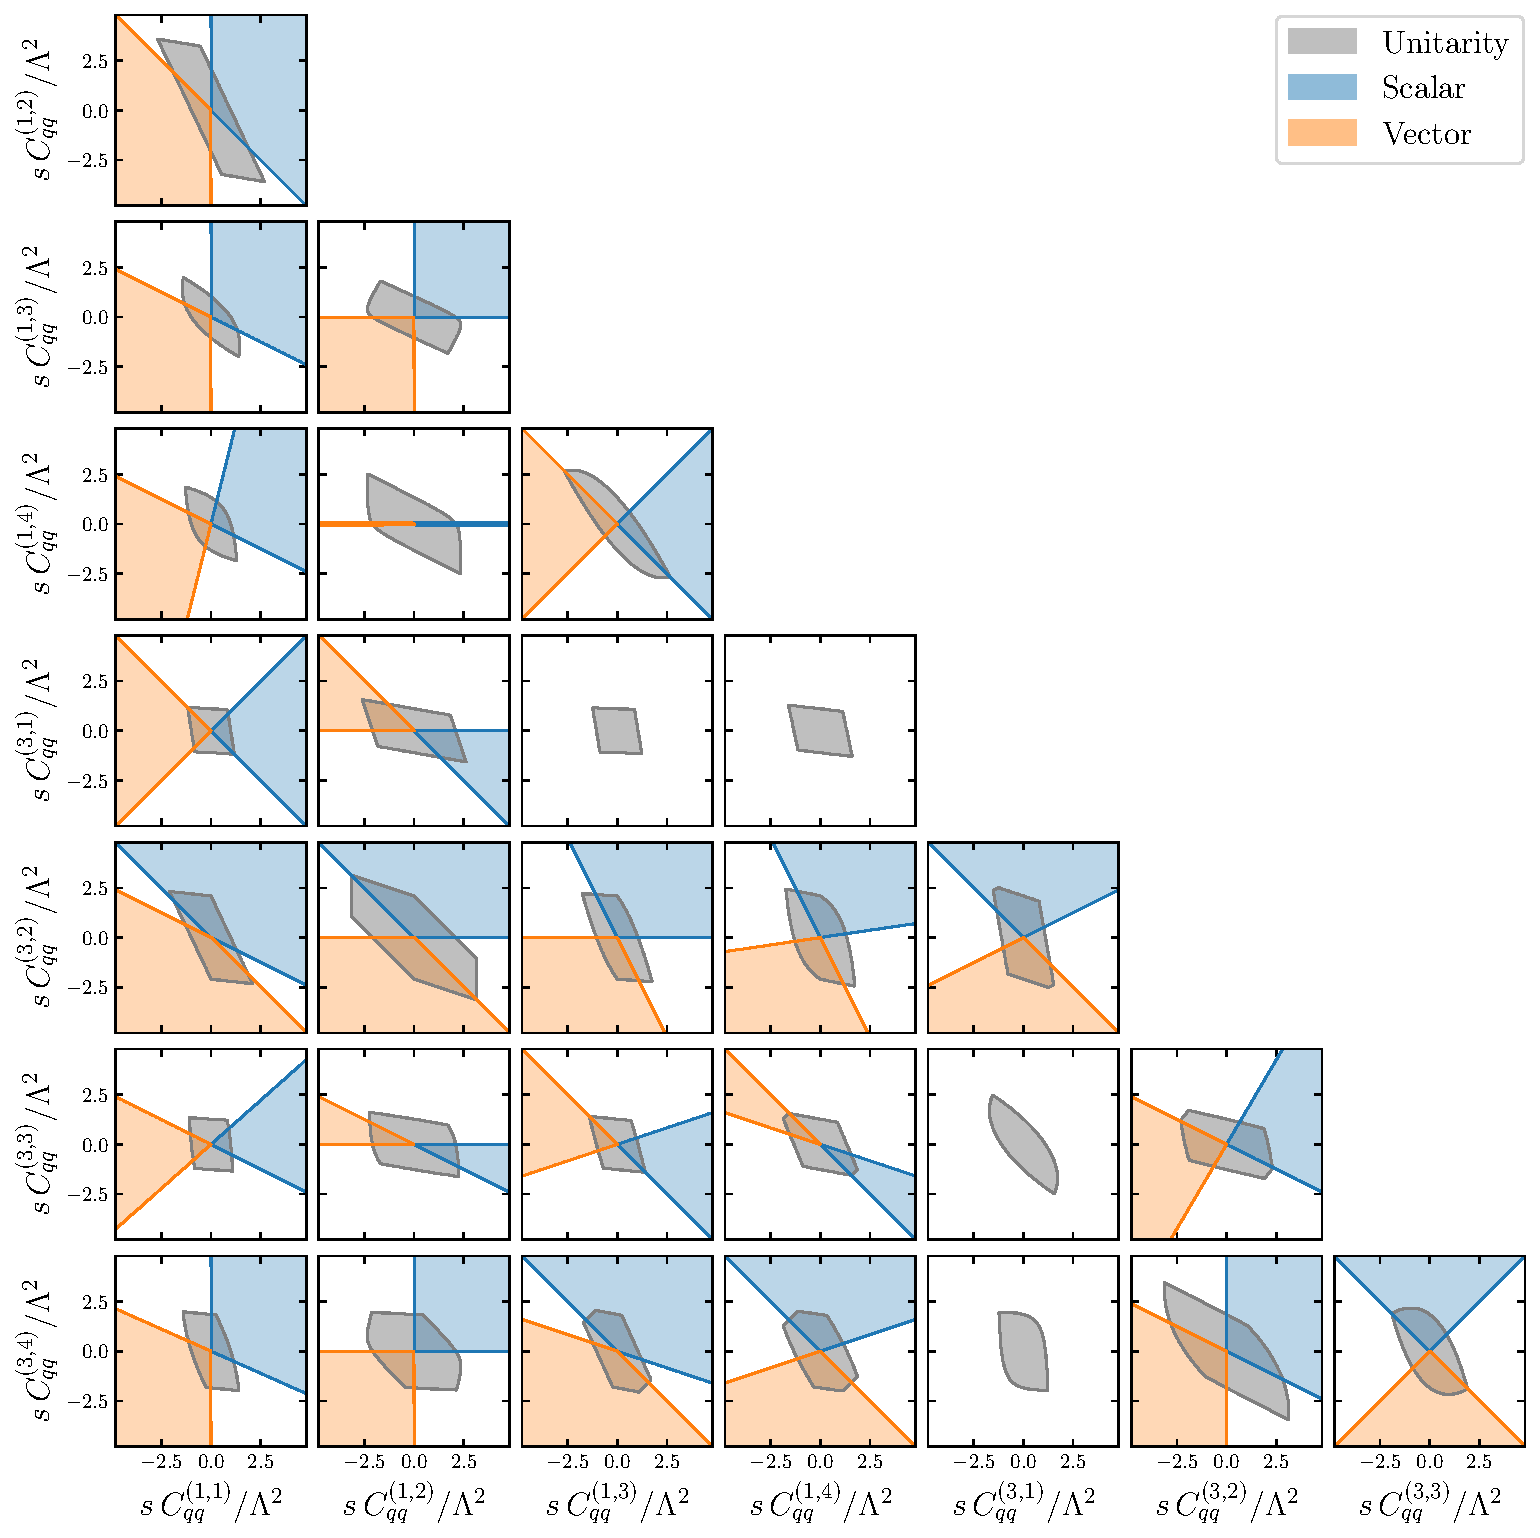
\includegraphics[width=1\linewidth]{images/flavor/Oqq_mfv.pdf}
    \caption{Partial-wave unitarity bounds and sum-rule constraints (under scalar and vector dominance) for the operators $O_{qq}^{(1,3)}$ under MFV, where $[C_{qq}^{(i)}]_{prst} =
            C_{qq}^{(i,1)}\delta_{pr}\delta_{st}
            + C_{qq}^{(i,2)}\delta_{pt}\delta_{sr}
            + C_{qq}^{(i,3)}((Y_u Y_u^\dagger)_{st}\delta_{pr} + (Y_u Y_u^\dagger)_{pr}\delta_{st}) + C_{qq}^{(i,4)}((Y_u Y_u^\dagger)_{sr}\delta_{pt} + (Y_u Y_u^\dagger)_{pt}\delta_{sr})$, $i=1,3$. The regions shown are two-dimensional slices of the full allowed region, obtained by setting to zero all the independent coefficients other than the two displayed.}
    \label{fig:Oqq_mfv}
\end{figure}

\begin{figure}[p]
    \centering
    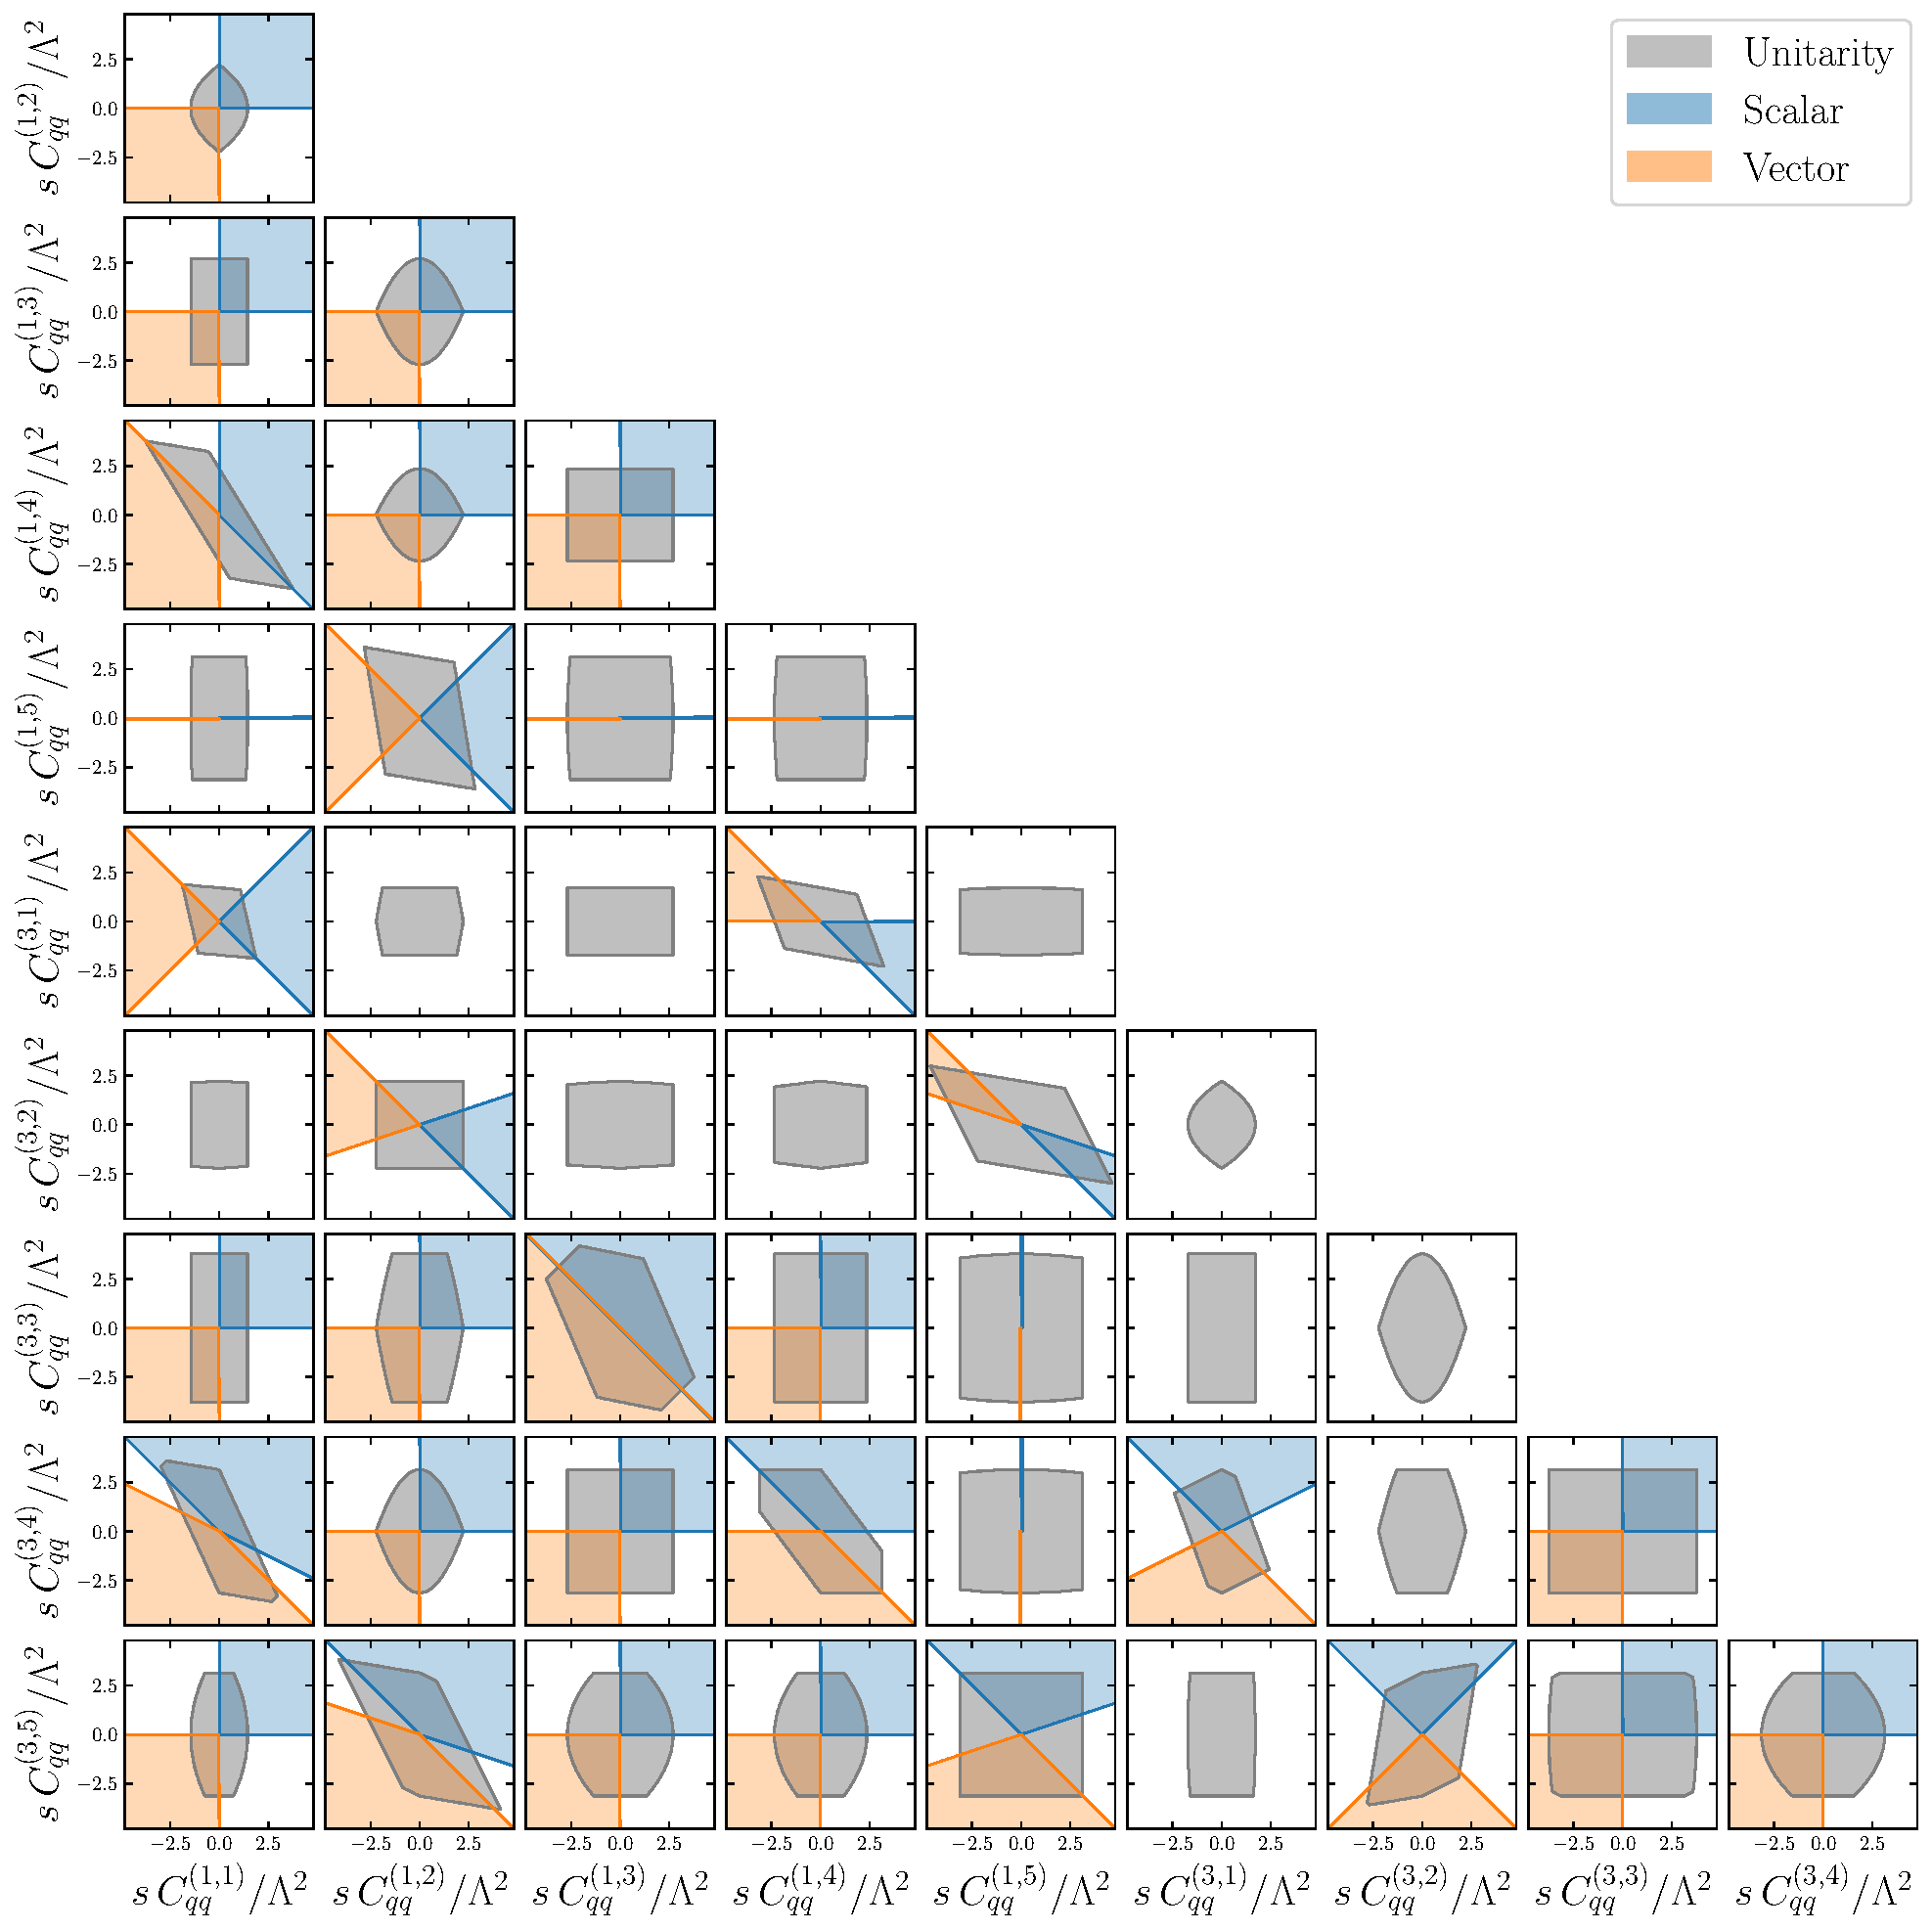
\includegraphics[width=1\linewidth]{images/flavor/Oqq_u2.pdf}
    \caption{Partial-wave unitarity bounds and sum-rule constraints (under scalar and vector dominance) for the operators $O_{qq}^{(i)}$ under $U(2)^5$ flavor symmetry, where $[C_{qq}^{(i)}]_{prst} =
            C_{qq}^{(i,1)}\Pij{p}{r}{a}\Pij{s}{t}{b}
            + C_{qq}^{(i,2)}(\Pij{s}{t}{a}\delta_{p3}\delta_{3r} + \Pij{p}{r}{a}\delta_{s3}\delta_{3t})
            + C_{qq}^{(i,3)}\delta_{p3}\delta_{3r}\delta_{s3}\delta_{3t}
            + C_{qq}^{(i,4)}\Pij{p}{t}{a}\Pij{s}{r}{b}
            + C_{qq}^{(i,5)}(\Pij{s}{r}{a}\delta_{p3}\delta_{3t} + \Pij{p}{t}{a}\delta_{s3}\delta_{3r})$, $i=1,3$. The regions shown are two-dimensional slices of the full allowed region, obtained by setting to zero all the independent coefficients other than the two displayed.}
    \label{fig:Oqq_u2}
\end{figure}

\begin{figure}[p]
    \centering
    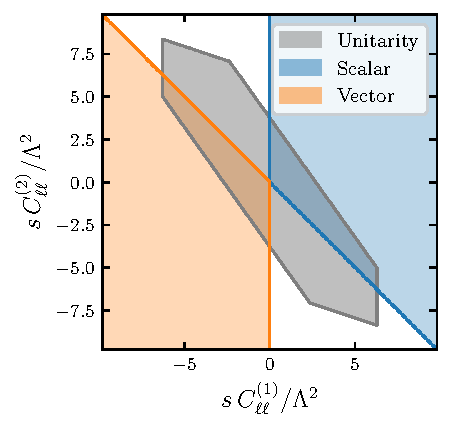
\includegraphics[scale = 0.75]{images/flavor/Oll_mfv.pdf}
    \caption{Partial-wave unitarity bounds and sum-rule constraints (under scalar and vector dominance) for the operator $O_{\ell\ell}$ under MFV, where $[C_{\ell\ell}]_{prst} = C_{\ell\ell}^{(1)}\delta_{pr}\delta_{st} + C_{\ell\ell}^{(2)}\delta_{pt}\delta_{rs}$.}
    \label{fig:Oll_mfv}
\end{figure}

\begin{figure}[p]
    \centering
    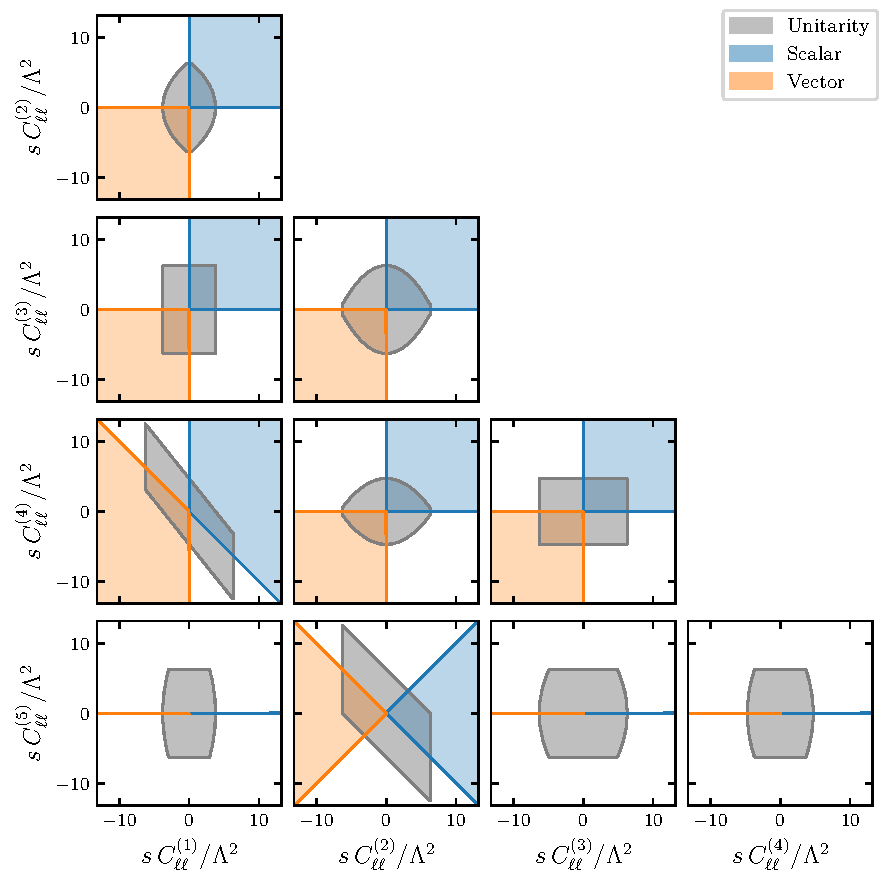
\includegraphics[scale = 0.75]{images/flavor/Oll_u2.pdf}
    \caption{Partial-wave unitarity bounds and sum-rule constraints (under scalar and vector dominance) for the operator $O_{\ell\ell}$ under $U(2)^5$ flavor symmetry, where $[C_{\ell\ell}]_{prst} =
            C_{\ell\ell}^{(1)}\Pij{p}{r}{a}\Pij{s}{t}{b}
            + C_{\ell\ell}^{(2)}(\Pij{s}{t}{a}\delta_{p3}\delta_{3r} + \Pij{p}{r}{a}\delta_{s3}\delta_{3t})
            + C_{\ell\ell}^{(3)}\delta_{p3}\delta_{3r}\delta_{s3}\delta_{3t}
            + C_{\ell\ell}^{(4)}\Pij{s}{r}{a}\Pij{p}{t}{b}
            + C_{\ell\ell}^{(5)}(\Pij{p}{t}{a}\delta_{s3}\delta_{3r} + \Pij{s}{r}{a}\delta_{p3}\delta_{3t})$. The regions shown are two-dimensional slices of the full allowed region, obtained by setting to zero all the independent coefficients other than the two displayed.}
    \label{fig:Oll_u2}
\end{figure}

\begin{figure}[p]
    \centering
    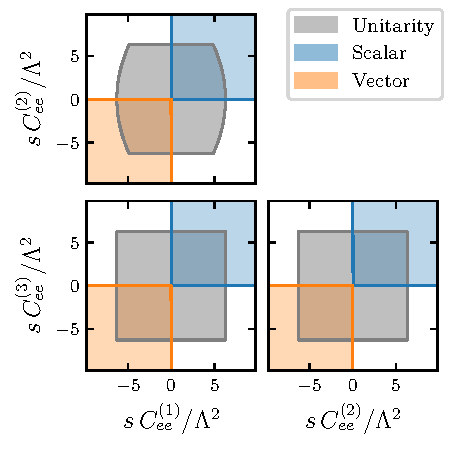
\includegraphics[scale = 0.75]{images/flavor/Oee_u2.pdf}
    \caption{Partial-wave unitarity bounds and sum-rule constraints (under scalar and vector dominance) for the operator $O_{ee}$ under $U(2)^5$ flavor symmetry, where $[C_{ee}]_{prst} =
            C_{ee}^{(1)}\Pij{p}{r}{a}\Pij{s}{t}{b}
            + C_{ee}^{(2)}(\Pij{s}{t}{a}\delta_{p3}\delta_{3r} + \Pij{p}{r}{a}\delta_{s3}\delta_{3t}) + C_{ee}^{(3)}\delta_{p3}\delta_{3r}\delta_{s3}\delta_{3t}$. The regions shown are two-dimensional slices of the full allowed region, obtained by setting to zero all the independent coefficients other than the two displayed.}
    \label{fig:Oee_u2}
\end{figure}

\begin{figure}[p]
    \centering
    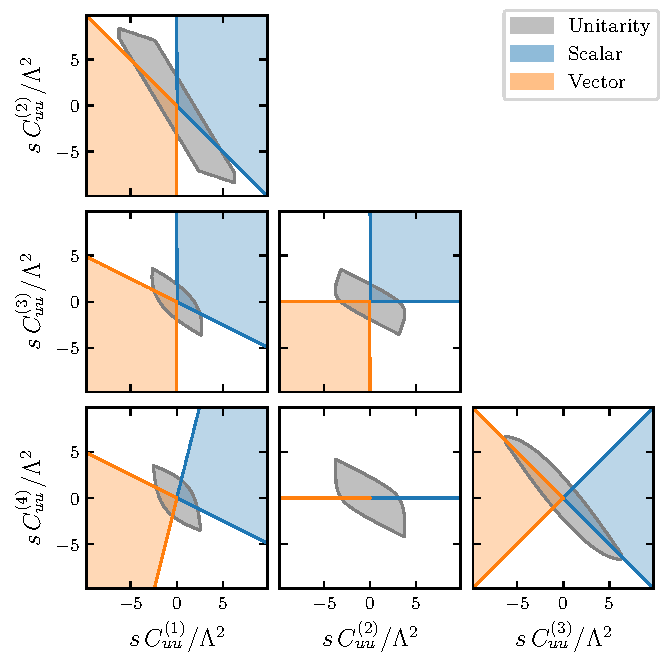
\includegraphics[scale = 0.75]{images/flavor/Ouu_mfv.pdf}
    \caption{Partial-wave unitarity bounds and sum-rule constraints (under scalar and vector dominance) for the operators $O_{uu}$ under MFV, where $[C_{uu}]_{prst} =
            C_{uu}^{(1)}\delta_{pr}\delta_{st}
            + C_{uu}^{(2)}\delta_{pt}\delta_{sr}
            + C_{uu}^{(3)}((Y_u^\dagger Y_u)_{st}\delta_{pr} + (Y_u^\dagger Y_u)_{pr}\delta_{st})+ C_{uu}^{(4)}((Y_u^\dagger Y_u)_{sr}\delta_{pt} + (Y_u^\dagger Y_u)_{pt}\delta_{sr})$. The regions shown are two-dimensional slices of the full allowed region, obtained by setting to zero all the independent coefficients other than the two displayed.}
    \label{fig:Ouu_mfv}
\end{figure}

\begin{figure}[p]
    \centering
    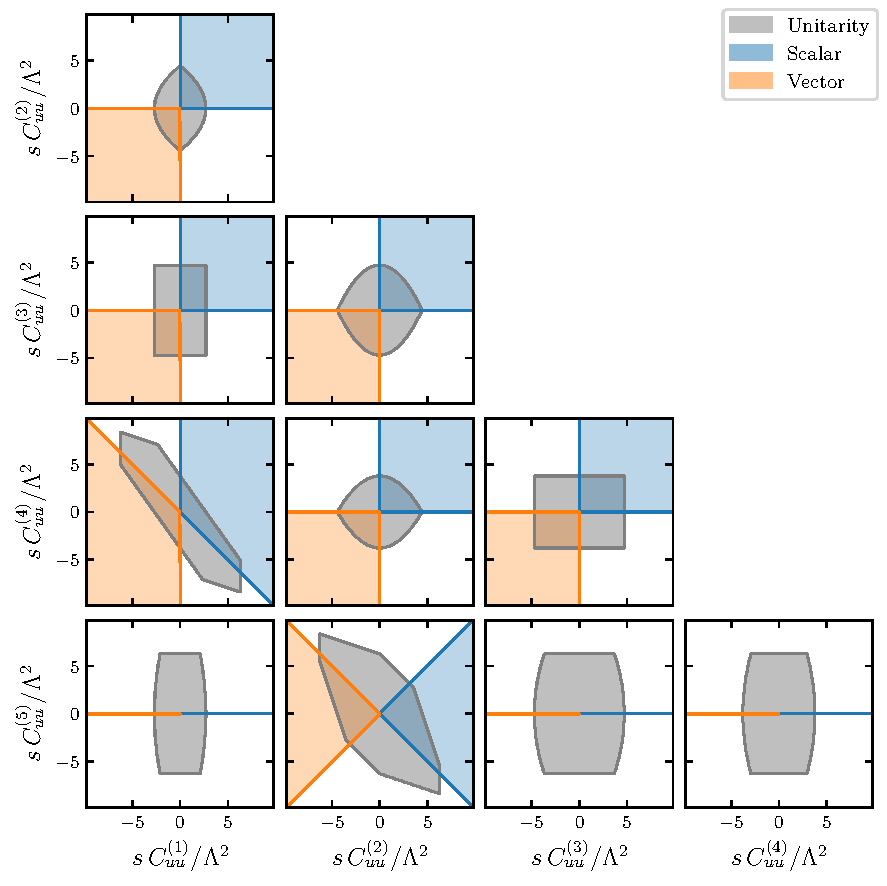
\includegraphics[scale = 0.75]{images/flavor/Ouu_u2.pdf}
    \caption{Partial-wave unitarity bounds and sum-rule constraints (under scalar and vector dominance) for the operators $O_{uu}$ under $U(2)^5$ flavor symmetry, where $[C_{uu}]_{prst} =
            C_{uu}^{(1)}\Pij{p}{r}{a}\Pij{s}{t}{b}
            + C_{uu}^{(2)}(\Pij{s}{t}{a}\delta_{p3}\delta_{3r} + \Pij{p}{r}{a}\delta_{s3}\delta_{3t})
            + C_{uu}^{(3)}\delta_{p3}\delta_{3r}\delta_{s3}\delta_{3t}
            + C_{uu}^{(4)}\Pij{p}{t}{a}\Pij{s}{r}{b}
            + C_{uu}^{(5)}(\Pij{s}{r}{a}\delta_{p3}\delta_{3t} + \Pij{p}{t}{a}\delta_{s3}\delta_{3r})$. Same decomposition and plots are valid also for $O_{dd}$. The regions shown are two-dimensional slices of the full allowed region, obtained by setting to zero all the independent coefficients other than the two displayed.}
    \label{fig:Ouu_u2}
\end{figure}

\begin{figure}[p]
    \centering
    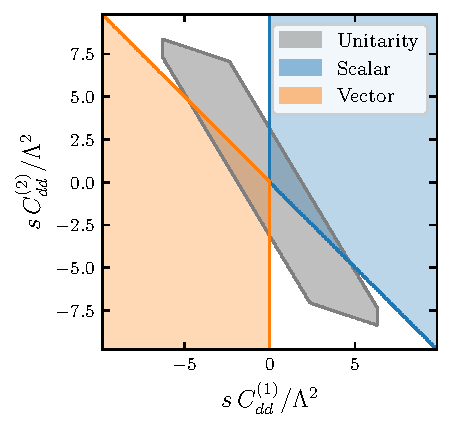
\includegraphics[scale = 0.75]{images/flavor/Odd_mfv.pdf}
    \caption{Partial-wave unitarity bounds and sum-rule constraints (under scalar and vector dominance) for the operators $O_{dd}$ under MFV, where $[C_{dd}]_{prst} =
            C_{dd}^{(1)}\delta_{pr}\delta_{st}
            + C_{dd}^{(2)}\delta_{pt}\delta_{sr}
            $.}
    \label{fig:Odd_mfv}
\end{figure}

\begin{figure}[p]
    \centering
    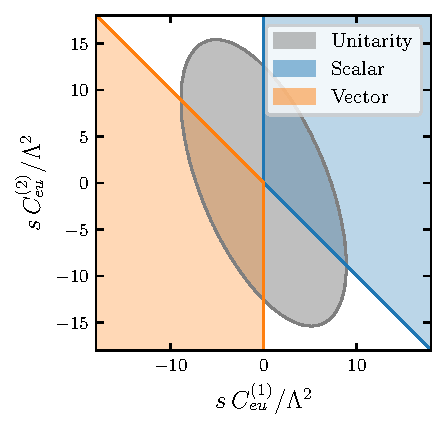
\includegraphics[scale = 0.75]{images/flavor/Oeu_mfv.pdf}
    \caption{Partial-wave unitarity bounds and sum-rule constraints (under scalar and vector dominance) for the operators $O_{eu}$ under MFV, where $[C_{eu}]_{prst} =
            C_{eu}^{(1)}\delta_{pr}\delta_{st}
            + C_{eu}^{(2)}\delta_{pr}(Y_u^\dagger Y_u)_{st}
            $.}
    \label{fig:Oeu_mfv}
\end{figure}

\begin{figure}[p]
    \centering
    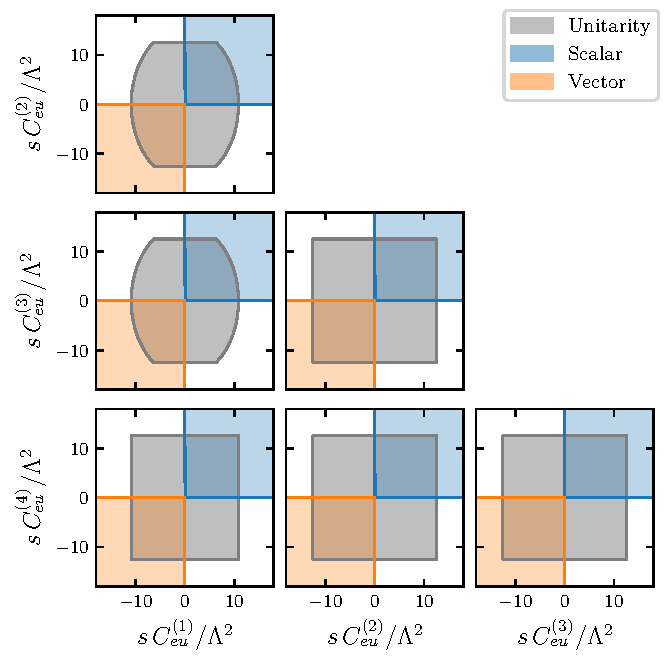
\includegraphics[scale = 0.75]{images/flavor/Oeu_u2.pdf}
    \caption{Partial-wave unitarity bounds and sum-rule constraints (under scalar and vector dominance) for the operators $O_{eu}$ under $U(2)^5$ flavor symmetry, where $[C_{eu}]_{prst} =
            C_{eu}^{(1)}\Pij{p}{r}{a}\Pij{s}{t}{b}
            + C_{eu}^{(2)}\delta_{p3}\delta_{3r}\Pij{s}{t}{a} + C_{eu}^{(3)}\delta_{s3}\delta_{3t}\Pij{p}{r}{a}
            + C_{eu}^{(4)}\delta_{p3}\delta_{3r}\delta_{s3}\delta_{3t}$. Same decomposition and plots are valid also for $O_{ed}$. The regions shown are two-dimensional slices of the full allowed region, obtained by setting to zero all the independent coefficients other than the two displayed.}
    \label{fig:Oeu_u2}
\end{figure}

\begin{figure}[p]
    \centering
    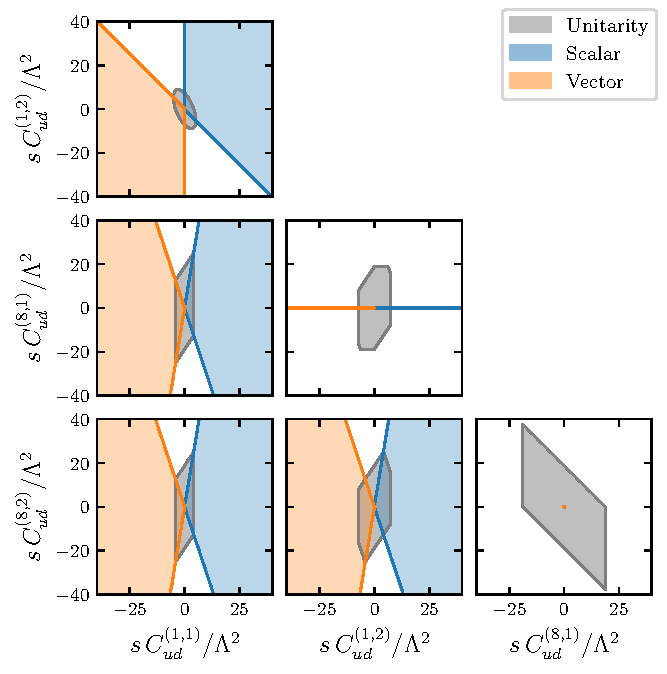
\includegraphics[scale = 0.75]{images/flavor/Oud_mfv.pdf}
    \caption{Partial-wave unitarity bounds and sum-rule constraints (under scalar and vector dominance) for the operators $O_{ud}^{(1,8)}$ under MFV, where $[C_{ud}^{(i)}]_{prst} =
            C_{ud}^{(i,1)}\delta_{pr}\delta_{st}
            + C_{ud}^{(i,2)}(Y_u^\dagger Y_u)_{pr}\delta_{st}$, $i=1,8$. The regions shown are two-dimensional slices of the full allowed region, obtained by setting to zero all the independent coefficients other than the two displayed.}
    \label{fig:Oud_mfv}
\end{figure}

\begin{figure}[p]
    \centering
    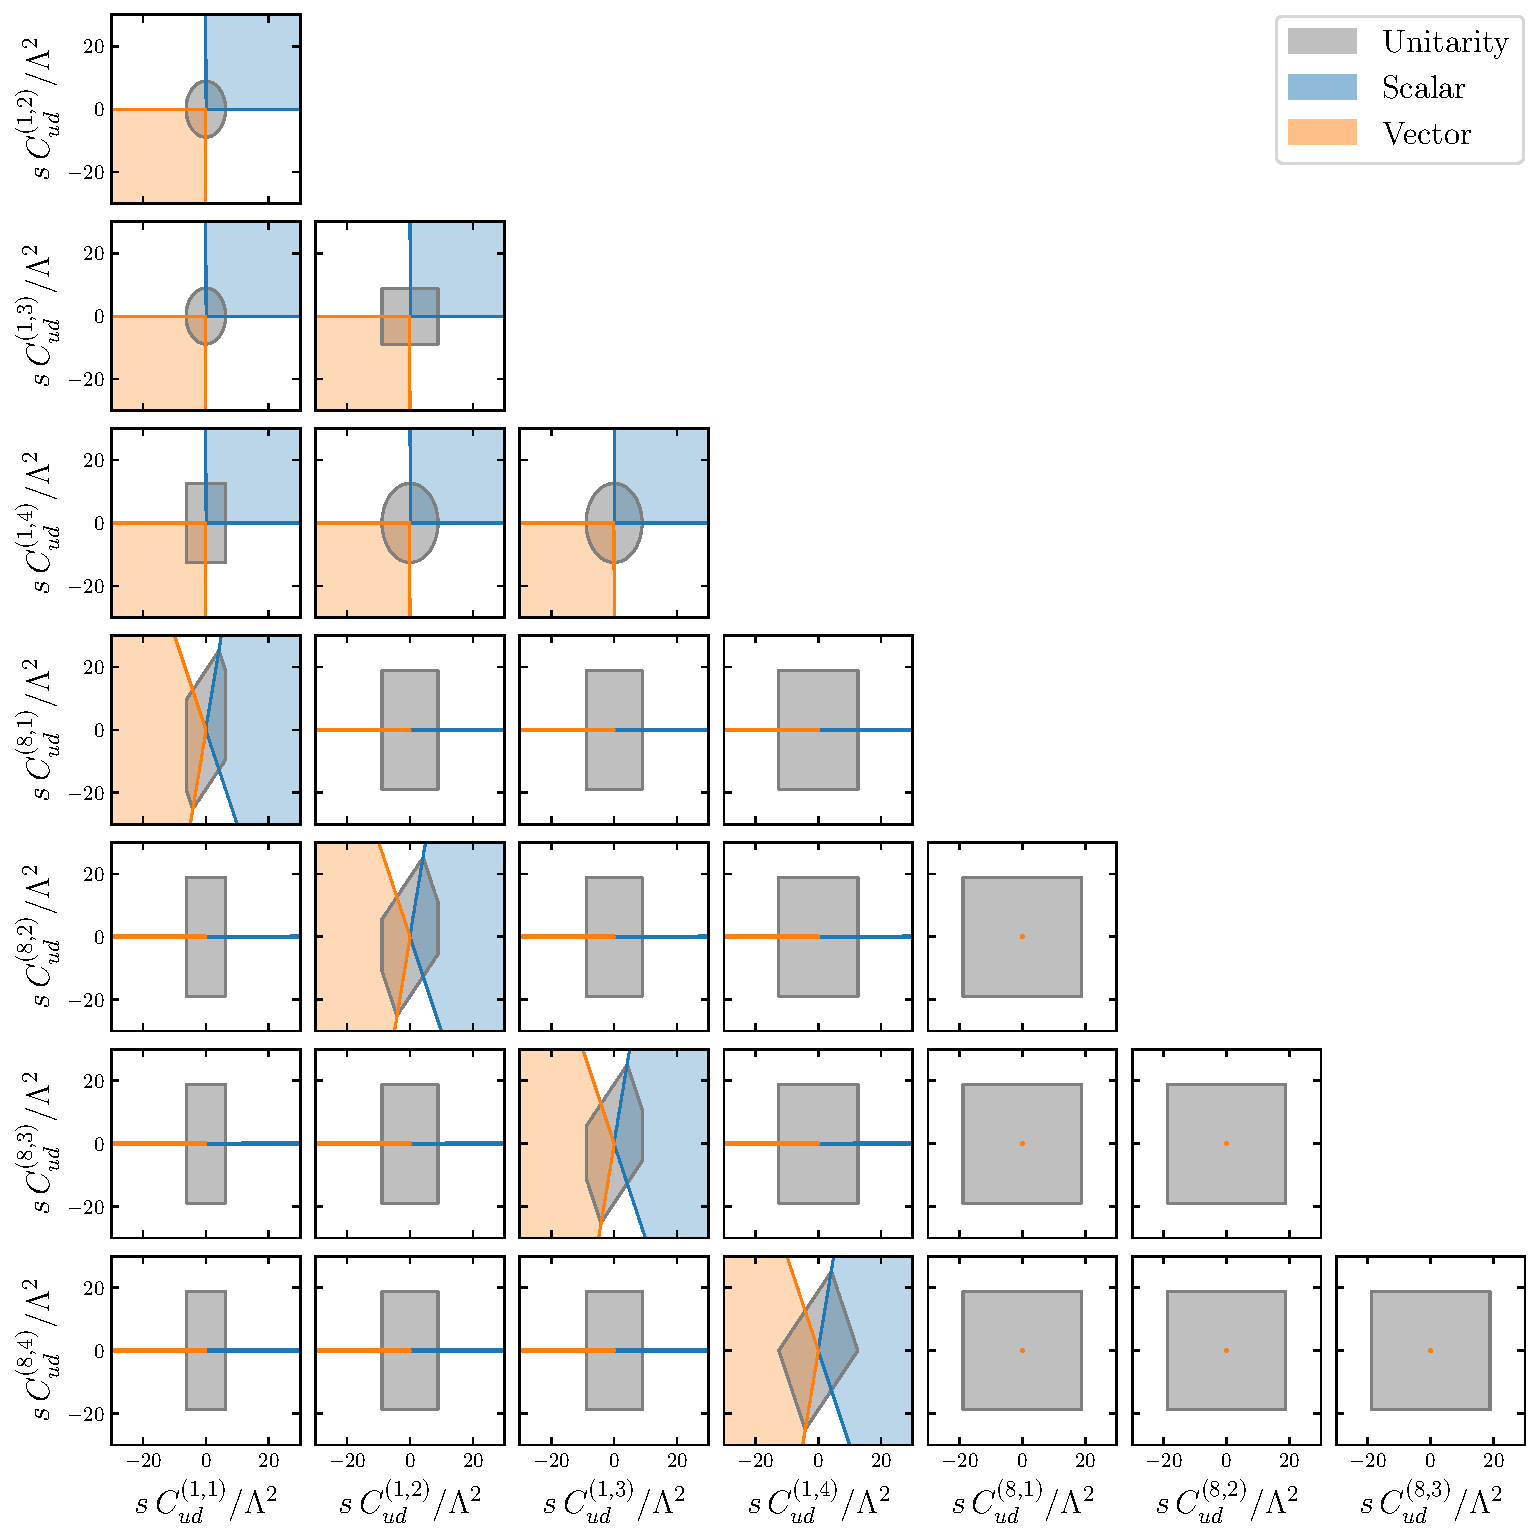
\includegraphics[width=\linewidth]{images/flavor/Oud_u2.pdf}
    \caption{Partial-wave unitarity bounds and sum-rule constraints (under scalar and vector dominance) for the operators $O_{ud}^{(1,8)}$ under $U(2)^5$ flavor symmetry, where $[C_{ud}^{(i)}]_{prst} =
            C_{ud}^{(i,1)}\Pij{p}{r}{a}\Pij{s}{t}{b}
            + C_{ud}^{(i,2)}\Pij{s}{t}{a}\delta_{p3}\delta_{3r}+ C_{ud}^{(i,3)}\Pij{p}{r}{a}\delta_{s3}\delta_{3t}
            + C_{ud}^{(i,4)}\delta_{p3}\delta_{3r}\delta_{s3}\delta_{3t}$, $i=1,8$. The regions shown are two-dimensional slices of the full allowed region, obtained by setting to zero all the independent coefficients other than the two displayed.}
    \label{fig:Oud_u2}
\end{figure}

\begin{figure}[p]
    \centering
    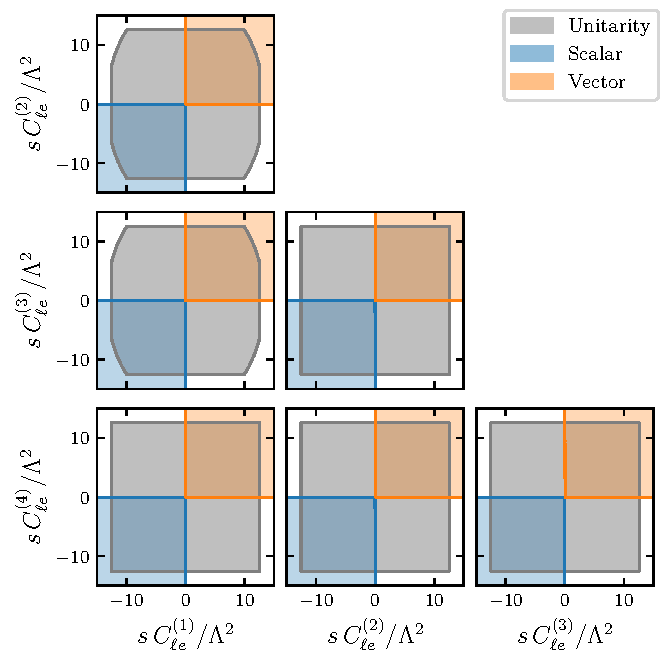
\includegraphics[scale = 0.75]{images/flavor/Ole_u2.pdf}
    \caption{Partial-wave unitarity bounds and sum-rule constraints (under scalar and vector dominance) for the operators $O_{\ell e}$ under $U(2)^5$ flavor symmetry, where $[C_{\ell e}]_{prst} =
            C_{\ell e}^{(1)}\Pij{p}{r}{a}\Pij{s}{t}{a}
            + C_{\ell e}^{(2)}\Pij{s}{t}{a}\delta_{p3}\delta_{3r}+ C_{\ell e}^{(3)}\Pij{p}{r}{a}\delta_{s3}\delta_{3t}
            + C_{\ell e}^{(4)}\delta_{p3}\delta_{3r}\delta_{s3}\delta_{3t}$. The regions shown are two-dimensional slices of the full allowed region, obtained by setting to zero all the independent coefficients other than the two displayed.}
    \label{fig:Ole_u2}
\end{figure}

\begin{figure}[p]
    \centering
    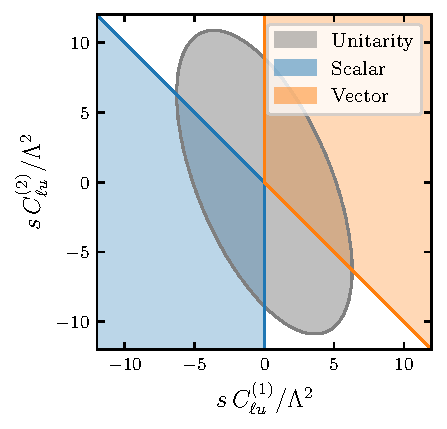
\includegraphics[scale = 0.75]{images/flavor/Olu_mfv.pdf}
    \caption{Partial-wave unitarity bounds and sum-rule constraints (under scalar and vector dominance) for the operators $O_{\ell u}$ under MFV, where $[C_{\ell u}]_{prst} = C_{\ell u}^{(1)}\delta_{pr}\delta_{st} + C_{\ell u}^{(2)}\delta_{pr}(Y_u^\dagger Y_u)_{st}$.}
    \label{fig:Olu_mfv}
\end{figure}

\begin{figure}[p]
    \centering
    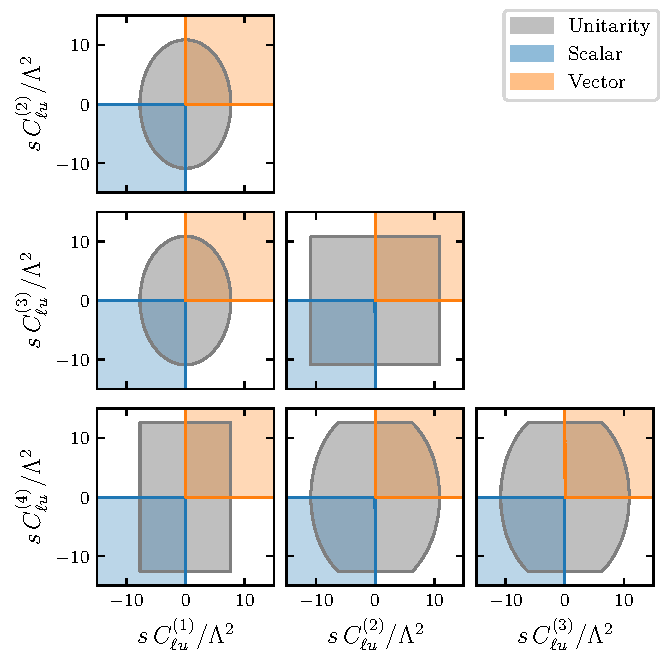
\includegraphics[scale = 0.75]{images/flavor/Olu_u2.pdf}
    \caption{Partial-wave unitarity bounds and sum-rule constraints (under scalar and vector dominance) for the operators $O_{\ell u}$ under $U(2)^5$ flavor symmetry, where $[C_{\ell u}]_{prst} =
            C_{\ell u}^{(1)}\Pij{p}{r}{a}\Pij{s}{t}{a}
            + C_{\ell u}^{(2)}\Pij{s}{t}{a}\delta_{p3}\delta_{3r}+ C_{\ell u}^{(3)}\Pij{p}{r}{a}\delta_{s3}\delta_{3t}
            + C_{\ell u}^{(4)}\delta_{p3}\delta_{3r}\delta_{s3}\delta_{3t}$. Same decomposition and plots are valid also for $O_{\ell d}$. The regions shown are two-dimensional slices of the full allowed region, obtained by setting to zero all the independent coefficients other than the two displayed.}
    \label{fig:Olu_u2}
\end{figure}

\begin{figure}[p]
    \centering
    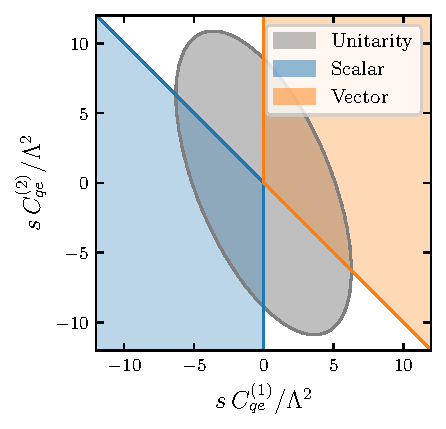
\includegraphics[scale = 0.75]{images/flavor/Oqe_mfv.pdf}
    \caption{Partial-wave unitarity bounds and sum-rule constraints (under scalar and vector dominance) for the operators $O_{qe}$ under MFV, where $[C_{qe}]_{prst} = C_{qe}^{(1)}\delta_{pr}\delta_{st} + C_{qe}^{(2)}(Y_u Y_u^\dagger)_{pr}\delta_{st}$.}
    \label{fig:Oqe_mfv}
\end{figure}

\begin{figure}[p]
    \centering
    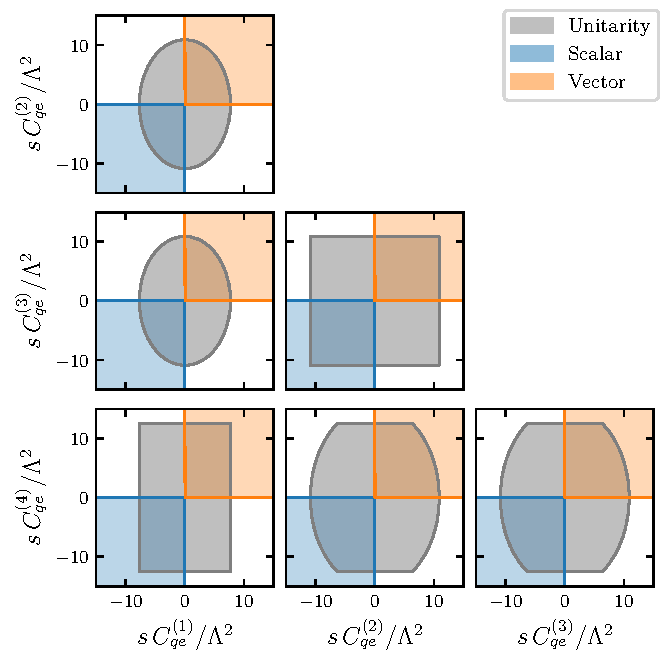
\includegraphics[scale = 0.75]{images/flavor/Oqe_u2.pdf}
    \caption{Partial-wave unitarity bounds and sum-rule constraints (under scalar and vector dominance) for the operators $O_{qe}$ under $U(2)^5$ flavor symmetry, where $[C_{qe}]_{prst} =
            C_{qe}^{(1)}\Pij{p}{r}{a}\Pij{s}{t}{a}
            + C_{qe}^{(2)}\Pij{s}{t}{a}\delta_{p3}\delta_{3r}+ C_{qe}^{(3)}\Pij{p}{r}{a}\delta_{s3}\delta_{3t}
            + C_{qe}^{(4)}\delta_{p3}\delta_{3r}\delta_{s3}\delta_{3t}$. The regions shown are two-dimensional slices of the full allowed region, obtained by setting to zero all the independent coefficients other than the two displayed.}
    \label{fig:Oqe_u2}
\end{figure}

\begin{figure}[p]
    \centering
    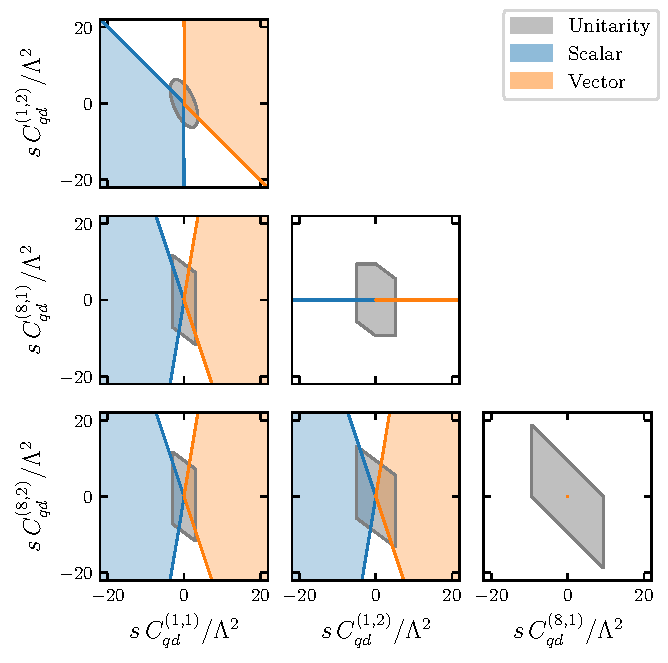
\includegraphics[scale = 0.75]{images/flavor/Oqd_mfv.pdf}
    \caption{Partial-wave unitarity bounds and sum-rule constraints (under scalar and vector dominance) for the operators $O_{qd}^{(1,8)}$ under MFV, where $[C_{qd}^{(i)}]_{prst} =
            C_{qd}^{(i,1)}\delta_{pr}\delta_{st}
            + C_{qd}^{(i,2)}(Y_u Y_u^\dagger)_{pr}\delta_{st}$, $i=1,8$. The regions shown are two-dimensional slices of the full allowed region, obtained by setting to zero all the independent coefficients other than the two displayed.}
    \label{fig:Oqd_mfv}
\end{figure}

\begin{figure}[p]
    \centering
    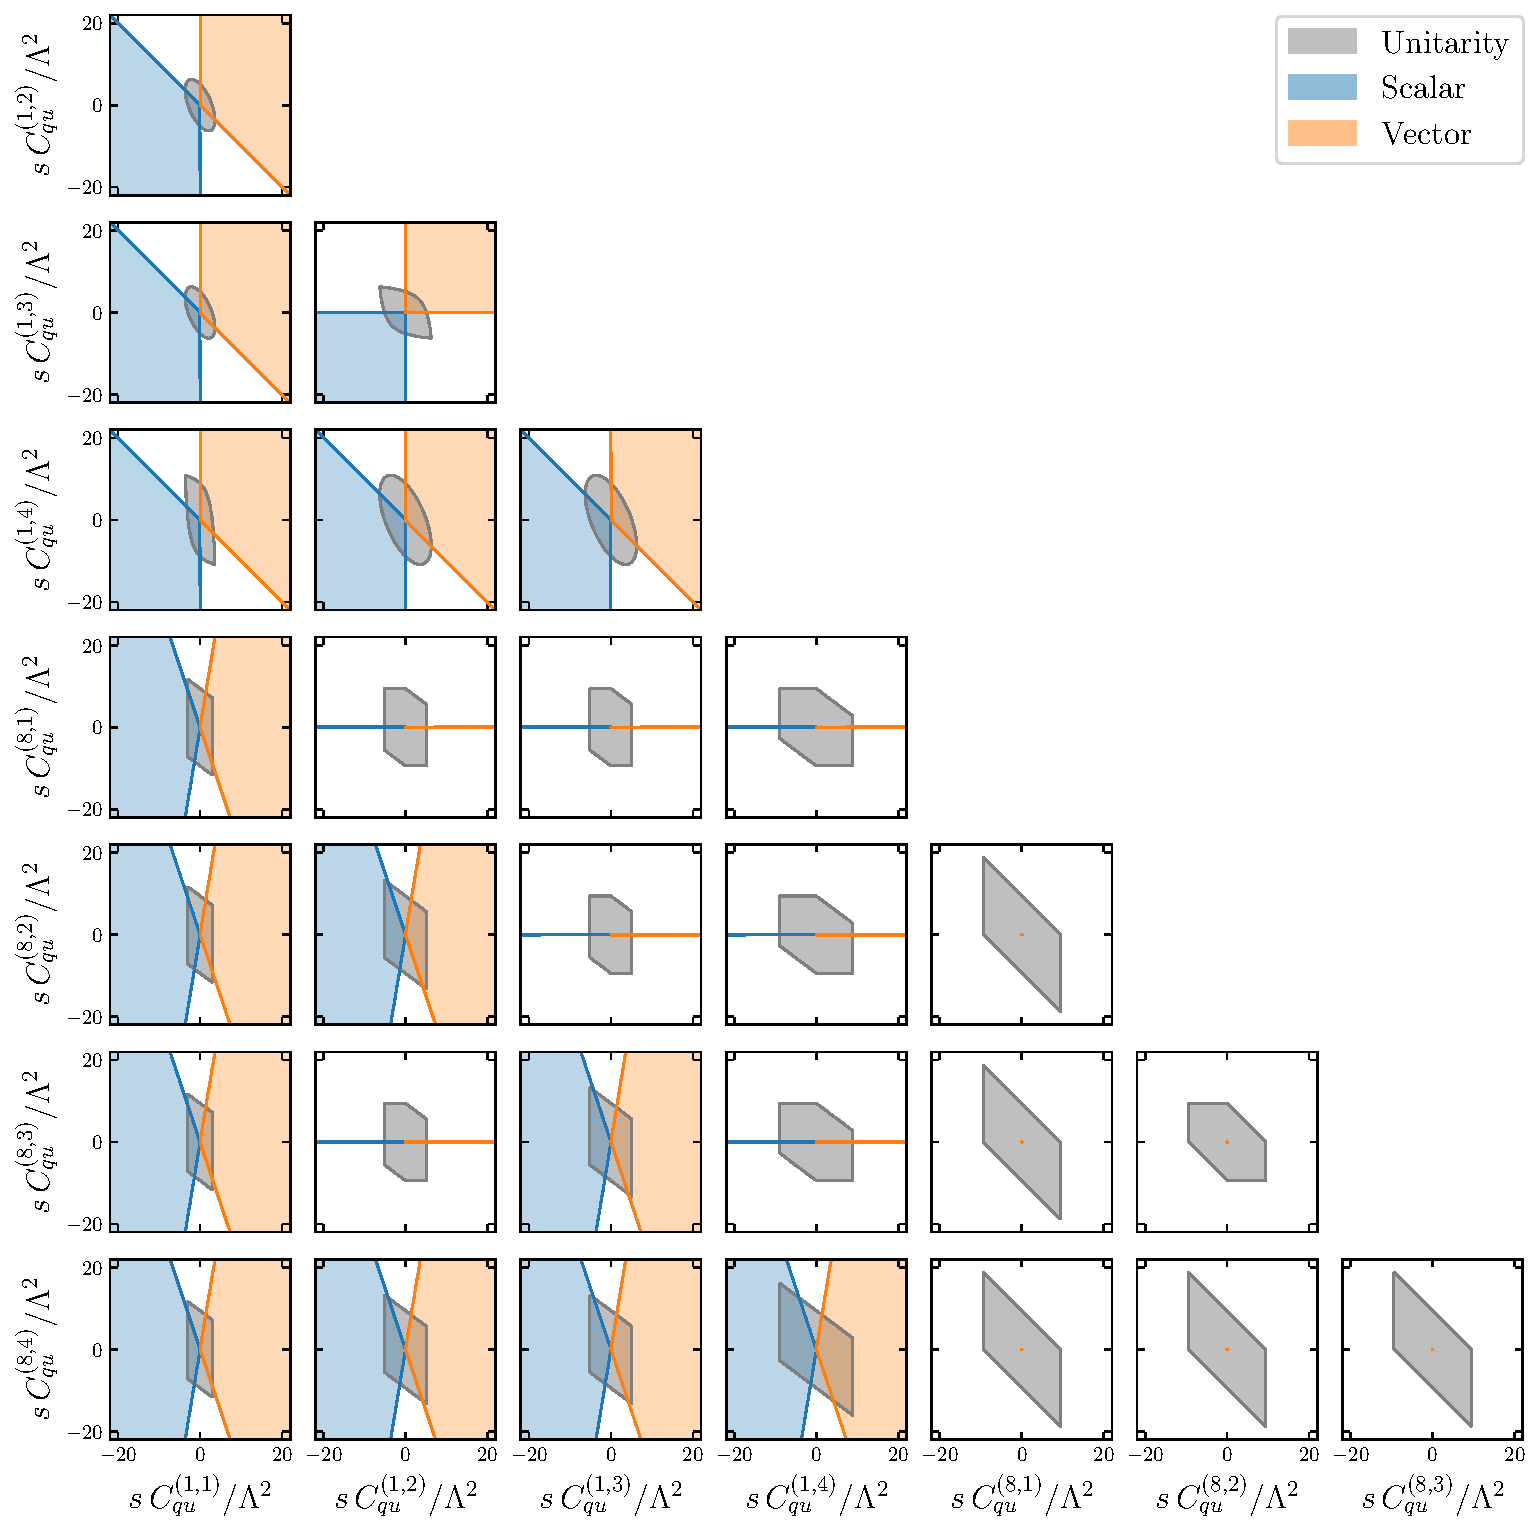
\includegraphics[width=\linewidth]{images/flavor/Oqu_mfv.pdf}
    \caption{Partial-wave unitarity bounds and sum-rule constraints (under scalar and vector dominance) for the operators $O_{qu}^{(1,8)}$ under MFV, where $[C_{qu}^{(i)}]_{prst} =
            C_{qu}^{(i,1)}\delta_{pr}\delta_{st}
            + C_{qu}^{(i,2)}(Y_u Y_u^\dagger)_{pr}\delta_{st}+ C_{qu}^{(i,3)}\delta_{pr}(Y_u^\dagger Y_u)_{st}
            + C_{qu}^{(i,4)}(Y_u)_{pt}(Y_u^\dagger)_{sr}$, $i=1,8$. The regions shown are two-dimensional slices of the full allowed region, obtained by setting to zero all the independent coefficients other than the two displayed.}
    \label{fig:Oqu_mfv}
\end{figure}

\begin{figure}[p]
    \centering
    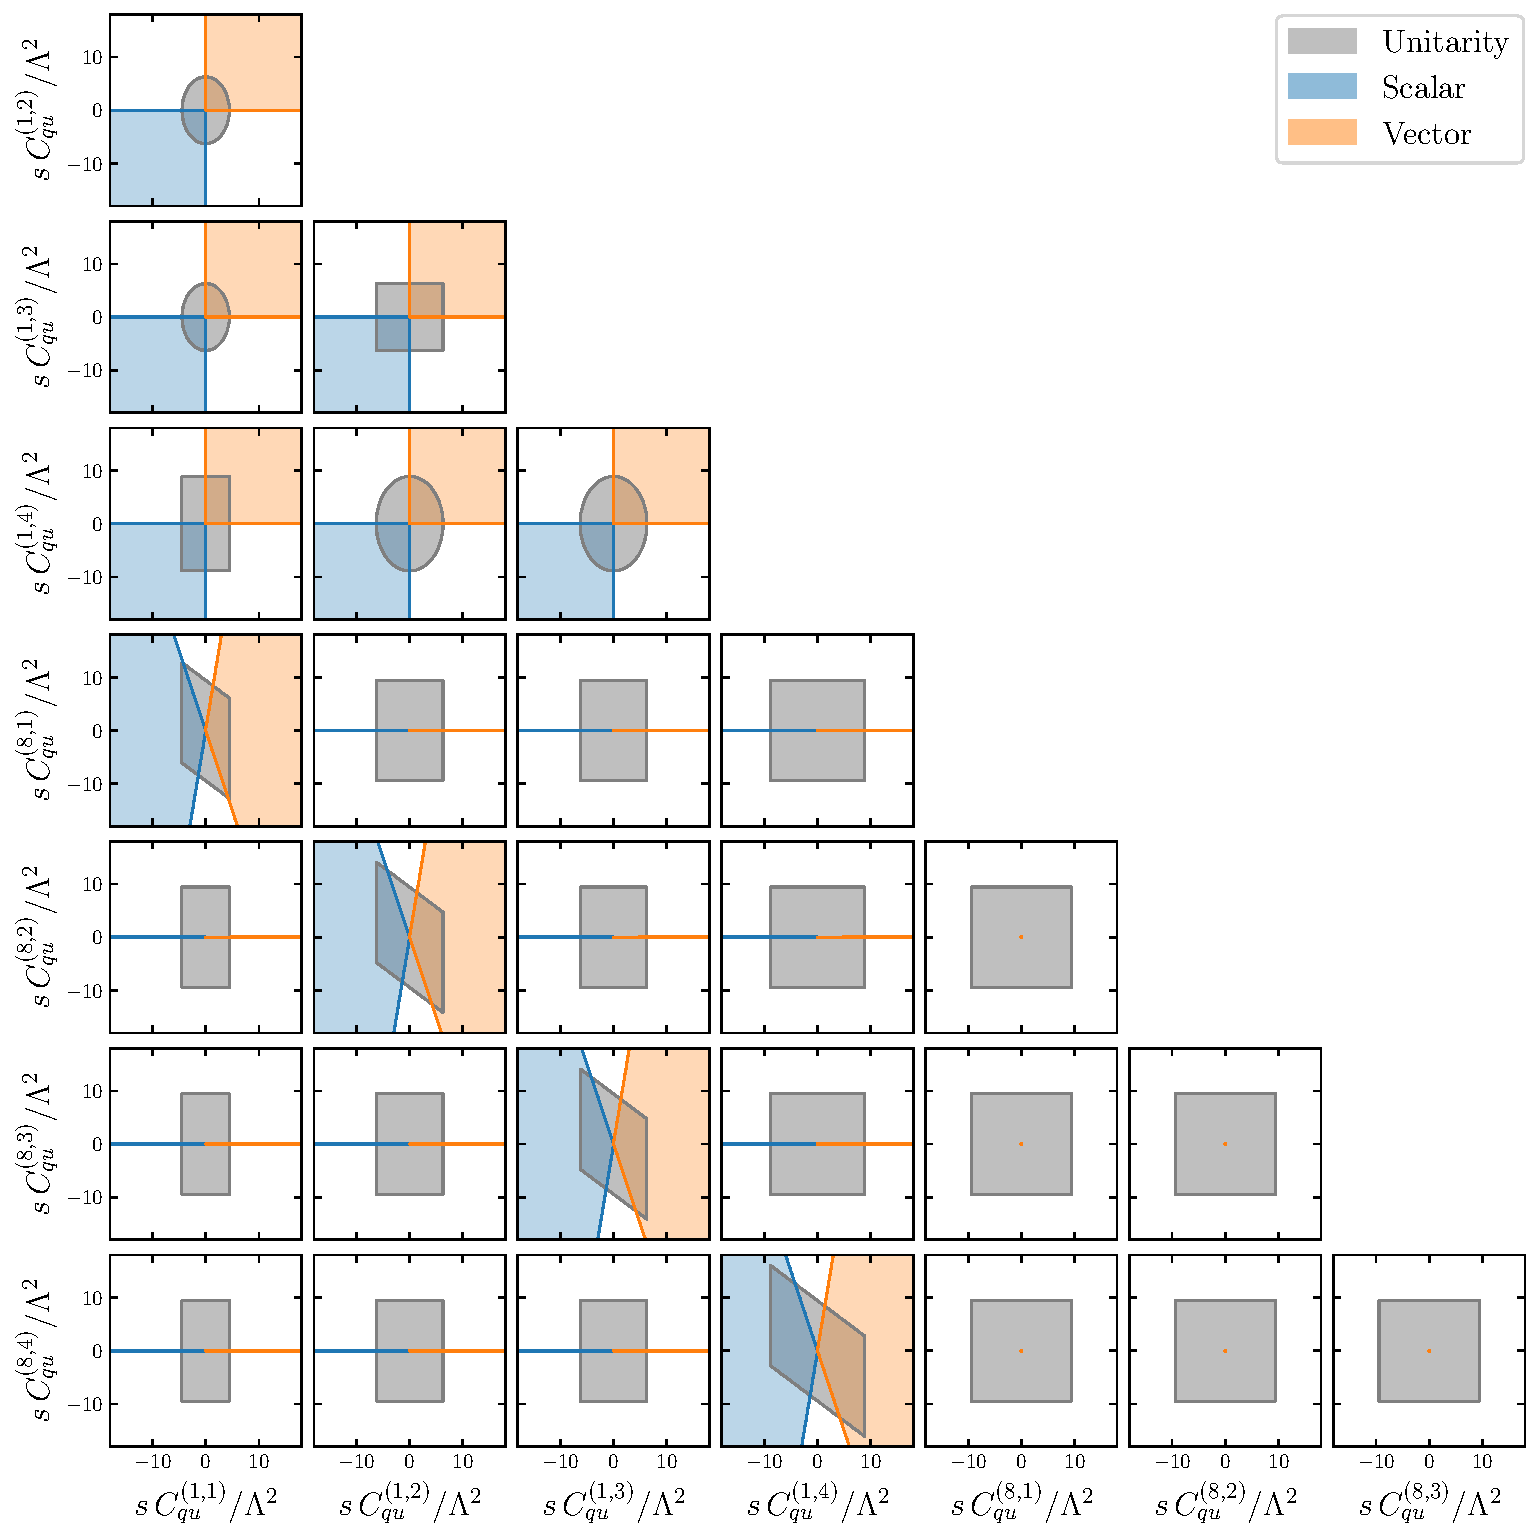
\includegraphics[width=\linewidth]{images/flavor/Oqu_u2.pdf}
    \caption{Partial-wave unitarity bounds and sum-rule constraints (under scalar and vector dominance) for the operators $O_{qu}^{(1,8)}$ under $U(2)^5$ flavor symmetry, where $[C_{qu}^{(i)}]_{prst} =
            C_{qu}^{(i,1)}\Pij{p}{r}{a}\Pij{s}{t}{a}
            + C_{qu}^{(i,2)}\Pij{s}{t}{a}\delta_{p3}\delta_{3r}+ C_{qu}^{(i,3)}\Pij{p}{r}{a}\delta_{s3}\delta_{3t}
            + C_{qu}^{(i,4)}\delta_{p3}\delta_{3r}\delta_{s3}\delta_{3t}$, $i=1,8$. Same decomposition and plots are valid also for $O_{qd}^{(1,8)}$. The regions shown are two-dimensional slices of the full allowed region, obtained by setting to zero all the independent coefficients other than the two displayed.}
    \label{fig:Oqu_u2}
\end{figure}
